\chapter{The Linux scheduler} %Capitolo in comune
\label{ch:sched}

As illustrated earlier, the CPU can only execute one task at a time and, even on multiprocessors systems, the number of tasks will be larger than the number of cores. For this reason, the scheduler is in charge of alternating the execution of tasks. % This is the job of the scheduler, which decides which task to run and for how long.
In order to decide which task to run and for how long, the scheduler has to consider many factors, such as
the importance of the task and its type.

\section{Introduction}%maybe to change

\subsection{Objectives of the scheduler}

The scheduler cannot simply choose the tasks in any order: there are some tasks that are highly time sensitive and need to be executed as fast as possible, and others that can wait longer without any consequence. This \textit{interactiveness} criteria is one of the most important aspects that the scheduler has to take into account.

%minimize response time and maximize throughput
\paragraph{Response time and throughput}
When interacting with the system, it's expected that it will react almost
immediately. Clearly, the user doesn't want to wait a second (or more)
between the pressure of a button and the response from the
system. Hence, the scheduler aims at detecting if the process
interacts with the user and tries to minimize the response time of such
processes.

%interactive tasks
There are different types of tasks: a text editor, for example, will spend most of its time waiting for user input, and when the input arrives, the task should respond as fast as possible. We call this kind of task \textit{interactive}. Other types of tasks, on the other hand, could utilize the CPU all the time without ever sleeping. %TODO example BATCH?
This means that the scheduler, not only needs to minimize the response time, but it should also give precedence to tasks that are highly interactive---especially on desktop systems.
%CPU bound vs IO bound

%throughput 
%MP: qui ho accorciato la spiegazione di context switch perchè l'ho stressato molto nel capitolo prima
Ideally, the scheduler should do as few process switches as possible. Preempting a task, choosing another one and then context switching is a long operation. Every time the scheduler is performing a context switch, the CPU is not being used by any task. This is why, on the long run, frequent context switches will have an impact on the performance of the system. More specifically, they will decrease the \textit{throughput}, which we define as the total amount of work completed per unit of time. It's important to note that we are talking about work done for the user: switching processes doesn't count as work since it's essentially overhead. Increasing the frequency of context switches would increase the responsiveness of the system, but it would also reduce the performance. The scheduler strives to find a balance between responsiveness and performance.

\paragraph{Fairness and Starvation}
Another important property that needs to be achieved is \textit{fairness}. What it means is that any two tasks with the same priority should run for roughly the same amount of time. Indeed, a task with higher priority should have the precedence over a task with a lower one, but at the same time, every task should get at least some CPU time. A process that doesn't get any CPU time is said to \textit{starve}. In practice, this usually happens when a process with high priority monopolizes a CPU, starving all the other processes waiting for their turn.

\subsection{Different workloads}  %https://lwn.net/Articles/230501/
Linux is used in all sorts of machines, from desktop computers to high-end servers to mobile devices. For this reason, the workload can vary a lot. Ideally, the scheduler should have good results in every scenario with every different workload, but in practice, this is really hard to implement. Even a small tweak to the scheduler could advantage desktop users over server users or viceversa: in other words, it's difficult to make every user happy.\cite{nice_design} Nonetheless, Linux tries to achieve flexibility by implementing scheduling classes. Ingo Molnar, the creator of the modern Linux scheduler, writes in the patch notes 
``[\dots Scheduling classes are] an extensible hierarchy of
scheduler modules. These modules encapsulate scheduling policy
details and are handled by the scheduler core without the core
code assuming about them too much.''\cite{ingo}. 
A task from a scheduling class can be chosen to run only if there are no runnable tasks in classes that are higher in the hierarchy. The scheduling classes are organized as shown in table \ref{tab:classes}, from high to low priority.

\begin{table}[t]
\centering
\begin{tabular}{|c|c|}
\hline
\textbf{Scheduling classes} & \textbf{Scheduling policies}\\
\hline
\texttt{stop\_sched\_class} &\\
\hline
\texttt{dl\_sched\_class}   & \texttt{SCHED\_DEADLINE}\\
\hline
\texttt{rt\_sched\_class}   & \texttt{SCHED\_FIFO} \\
                   		   & \texttt{SCHED\_RR}\\
\hline
\texttt{fair\_sched\_class} & \texttt{SCHED\_NORMAL}\\
                   & \texttt{SCHED\_BATCH}\\
                   & \texttt{SCHED\_IDLE}\\
\hline
\texttt{idle\_sched\_class} &\\          
\hline
\end{tabular}
\caption{Scheduling classes and policies in Linux}\label{tab:classes}
\label{tab:sched_classes}
\end{table}
\paragraph{Classes and policies}
Each class has its code, implementing its own algorithm. Within each class, policies represent special scheduling decisions, and each process has a policy associated with it. This means that at specific points of the code the behavior may change depending on the process' policy. This may seem confusing, but consider \verb|SCHED_RR| and \verb|SCHED_FIFO|: they use the same priority scale, so processes of both policies share the same run queues. Furthermore, FIFO and round-robin are very similar algorithms, differing just because of round-robin having time quantums. From this perspective, it makes sense that tasks of both policies are scheduled using the same code. Scheduling classes are mapped to their code as follows:
\begin{itemize}
\item \verb|dl_sched_class| -- \verb|kernel/sched/deadline.c|
\item \verb|rt_sched_class| -- \verb|kernel/sched/rt.c|
\item \verb|fair_sched_class| -- \verb|kernel/sched/fair.c|
\end{itemize}
\verb|SCHED_DEADLINE| is the highest priority policy. A task with this policy defines a deadline, before which the task has to finish its execution. The scheduler guarantees that the deadline is respected. To do that, when the policy or the attributes are changed, the scheduler checks the feasibility of the change, and if the CPU is too busy then it returns an error.
\verb|SCHED_FIFO| is a cooperative policy, first come first served: the tasks are executed in the order of arrival, and there is no notion of timeslice. Even if FIFO is cooperative in principle, \verb|SCHED_FIFO| allows preemption. In fact, all scheduling on Linux is peemptive. A running task with this policy can be preempted if another task with higher priority becomes runnable.
\verb|SCHED_RR| is a round-robin policy. It's similar to \verb|SCHED_FIFO| but it uses round-robin to cycle trough all the tasks with the same priority. Each task can run only for a maximum fixed timeslice (quantum of time) then it's preempted and put at the end of list of its priority. As for \verb|SCHED_FIFO|, if a higher priority task becomes runnable, the current task is preempted.
\verb|SCHED_NORMAL| is the default policy that is used for regular tasks and uses CFS (the Completely Fair Scheduler, implemented in \verb|fair.c|), this chapter later describes how it works. Most tasks run with this priority on most systems.
\verb|SCHED_BATCH| is similar to \verb|SCHED_NORMAL| but it will preempt less frequently, so every process will run longer. For this reason, it is more suited for non-interactive workloads, typically on servers.
\verb|SCHED_IDLE| is for tasks with very low priority, almost any task can preempt tasks with this policy.

\paragraph{Priorities} %TODO static and dynamic priorities
Each task has a priority associated with it, the first priority levels
corresponds to real-time tasks and are scheduled with the
\verb|SCHED_FIFO| or \verb|SCHED_RR| policy. Normal tasks are
scheduled with the \verb|SCHED_NORMAL|, \verb|SCHED_BATCH| and
\verb|SCHED_IDLE|, these have a priority (called nice) that ranges
from $-20$ to $19$, $-20$ being the highest priority and $+19$ the
lowest. The behaviour of different nice values depends on the version
of the scheduler.

%EXTRA PARAGRAPH?
%this has been a problem for linux for years (advantaging servers)
%today, tweaks are needed to optimize for a workload

\label{sec:cfs}
\section{Prior to CFS}
The \textit{Completely Fair Scheduler} (CFS) is the default scheduler of Linux since the 2.6.23 release, as a replacement for the $O(1)$ scheduler. To understand the advantages of CFS, it is important to understand how the previous scheduler works.

\subsection{The $O(1)$ Scheduler}
In the $O(1)$ scheduler, runnable tasks are stored in two priority queues (\textit{run queues}): an active and an expired queue. Initially, all the tasks are inside the active queue. Then, the tasks run on the CPU, in order of priority, for the assigned timeslice: when it expires, the task is moved into the expired queue. Once all the tasks have finished their timeslice, the two queues swap roles and the process starts again.

Prior to the introduction of the O(1) scheduler, there was another version of the scheduler that was much simpler. It worked well with a small number of tasks, but there were performance issues when working with many tasks. When the $O(1)$ scheduler was introduced its goal was to keep all the positive aspects of the previous scheduler, like good interactive performance and fairness, but improving the scalability. That is, improving the performance when dealing with a large number of tasks.
This was achieved using only algorithms with constant complexity $O(1)$. Meaning that the $O(1)$ scheduler does not have to traverse all the list of runnable tasks when deciding which one to run. Instead, this decision always takes a constant amount of time, regardless of the number of tasks.

\paragraph{Priority} %What is the priority of a task
Each user task has a priority which consists of a static and a bonus priority. The static priority, which corresponds to the \textit{nice} value, can have a value from $-20$ to $19$, $-20$ being the highest priority and 19 the lowest. The bonus ranges from $-5$ to $+5$ and it is determined by the interactiveness of the task: if a task spends a large amount of time sleeping, the scheduler will boost its priority, on the other hand, if a task doesn't sleep much, it will get penalized. %TODO explain nice meaning
The static priority and the bonus are then added to determine the dynamic priority, which is the priority looked by the scheduler when choosing the next process to run.

\paragraph{Timeslice} %How are timeslices calulated
The $O(1)$ scheduler is based on the concept of timeslice, this is the amount of time that a task runs on the CPU during a cycle. A new cycle begins when every task has been moved to the expired queue. Each priority level is mapped to a different timeslice: higher levels get mapped to more time while lower levels get mapped to less time. The timeslice can be expressed as a time quantity, but it's more usual to represent it as a percentage of the total time of a cycle.

%http://ijssst.info/Vol-15/No-3/data/3857a668.pdf Cita questo (on the fairness of O(1))
\paragraph{Interactive tasks and heuristics} %TODO talk about heuristics! (sleep time etc)
A process that is marked as interactive will be reinserted in the
active queue after it has expired its current timeslice. This is done 
to improve the response time of the system. A task is
marked as interactive depending on its dynamic priority and its nice
value. It is easier for a task with an higher priority to become interactive compared to task with a lower one. A task with a nice value of $-20$ it's marked as interactive
even if it has a dynamic priority of $+3$, while a task with a nice
value of $0$ has to have a dynamic priority of $-2$. With a nice level
of $+19$ it is impossible for a task to be marked as interactive, independently from the dynamic priority. %hardcoded values, arbitrary

This system is the biggest weakness of the O(1) scheduler: it generated unpredictable behavior and could cause some tasks to be marked as interactive even when they were not. Furthermore, the different kinds of complex heuristics made the code bigger and harder to understand and maintain.

% www.kernel.org/doc/Documentation/scheduler/sched-nice-design.txt
\paragraph{Nice levels} 
Prior to the introduction of the $O(1)$ scheduler, tasks with a nice of 19 were using too much CPU and users were complaining.\cite{nice_design} Because of this, $O(1)$ was specifically designed to have the minimum timeslice set to one \textit{jiffy}, which is the minimum measurable amount of time.  
\begin{figure}[t] %how do i place it in the right position?
  \centering
  \begin{tikzpicture}
    \begin{axis}[ xlabel = nice,
      ylabel = timeslice (ms)]
      \addplot[domain=-20:0, color=red] {20*(140-(120+x))};
      \addplot[domain=0:19, color=green] {4*(140-(120+x))};
    \end{axis}
  \end{tikzpicture}
  \caption{Nice to timeslice conversion}
  \label{fig:timeslice_vs_nice}
\end{figure}%SC: to verify, that "jump" is odd, but the code for the old scheduler seems to confirm it.
The amount of time corresponding to one jiffy depends on the tick
rate. In the kernel, the tick rate is the constant \verb|HZ|, which is defined as the number of ticks per second. Despite the name, this value is not tied to the processor's frequency. 
With the advancements of
computer hardware, this value increased, and today it's usually 1000 on desktop computers. With such a value, a jiffy is equivalent to 1 msec, meaning that a task with nice $+19$
would get a timeslice of only 1 msec (only 0.1\% CPU time) and this would cause too frequent
rescheduling, causing problems like cache trashing. The value of the
minimum timeslice can be adjusted, but it is still \verb|HZ| dependent. More
details on this topic can be found in Section~\ref{sec:timekeeping}.

%Magari spiegare meglio usando www.kernel.org/doc/Documentation/scheduler/sched-nice-design.txt
Another problem, that can be noticed in the graph of
Figure~\ref{fig:timeslice_vs_nice}, is that the behavior of the nice
level depends on its absolute value. But the nice API only allows the nice to be changed by a relative amount. 
This means that with the $O(1)$ scheduler, calling \verb|nice(1)| to increment the nice level of a task has different effects depending on the initial value. 

The last problem was that tasks with negative nice values were not responsive enough: this was problematic for multimedia applications, which had to resort to run under \verb|SCHED_FIFO| rather than \verb|SCHED_NORMAL|. This approach caused another major problem because \verb|SCHED_FIFO|, as we stated earlier, is not starvation proof.

\subsection{Rotating Staircase DeadLine}
Con Kolivas proposed a new scheduler that tries to solve the problems of the $O(1)$ scheduler. The goal was to design a scalable scheduler that was completely fair to all processes while allowing the best possible interactivity.\cite{con}

The \textit{Rotating Staircase DeadLine scheduler} (RSDL) assigns a quota of
runtime based on the priority of the task. The tasks at the highest
priority level are then executed round-robin with each other. When a
task finishes its quota, it is moved to the next priority level and it
is given a new quota. The entire priority level also has an assigned
quota, when that quota expires, all the process in that priority level
are moved to the next one. When a task finishes all its quotas at each
priority level, it is moved to the expired queue, then, when all the tasks
have finished their quota, the expired queue becomes active and the
process starts again.

RSDL doesn't measure the sleep time of the tasks to identify interactive tasks. Tasks that spend most of the time sleeping will consume a little portion of their quota. When they get woken up, they will probably be at a high priority level. Meaning that, in most cases, they only have to wait for the task that is currently running. This guarantees a low latency for interactive tasks, which will rise to high priorities in a natural way, getting rid of the heuristics. 

\section{Completely Fair Scheduler (CFS)}
The RDSL scheduler never made it into the kernel, but the CFS scheduler, which was developed by Ingo Moln\'ar\cite{ingo}, was inspired by RSDL.

Like RSDL, CFS does not use fixed timeslices and does not use any heuristic
method to calculate the priority of a task. It tries to model an ideal
multitasking CPU on real hardware. Ideally every task receives
$\frac 1n$ of the processor's time, with $n$ being the number of
runnable tasks. This results in simpler code that can handle nice
values better than the previous scheduler; the preemption time is no
longer fixed like in the $O(1)$ scheduler, but it is variable.\cite{cfs_design} This approach solves the problem found in the $O(1)$ scheduler: the behaviour of nice levels is more consistent and independent from the tick-rate; increasing the nice value by one has the same effect regardless of the starting value. Each process gets
assigned a portion of the CPU depending on its weight, which is
determined by the nice of the task. %and the vruntime?
%in CFS there is much more difference between SCHED_NORMAL and SCHED_BATCH ... \cite{ingo}

\subsection{Weight function}
According to the comments in the code of \verb|kernel/sched/core.c|, and the kernel documentation, the weight $w$ is roughly equivalent to
\begin{equation}
  w(n) = \dfrac{1024}{(1.25)^{n}}.
  \label{eq:weight_nice}
\end{equation}
with $n$ being the nice of the task, and 1024 being the weight of a task with nice 0. To avoid computing this function every time it is needed, there is a pre-calculated table which maps nice
values to the corresponding weight. Below, the code from
\verb|kernel/sched/core.c| is reported. In this code fragment, the developer's comments are useful
to understand how this formula works.
\begin{code}
/*
 * Nice levels are multiplicative, with a gentle 10% change for every
 * nice level changed. I.e. when a CPU-bound task goes from nice 0 to
 * nice 1, it will get ~10% less CPU time than another CPU-bound task
 * that remained on nice 0.
 *
 * The "10% effect" is relative and cumulative: from _any_ nice level,
 * if you go up 1 level, it's -10% CPU usage, if you go down 1 level
 * it's +10% CPU usage. (to achieve that we use a multiplier of 1.25.
 * If a task goes up by ~10% and another task goes down by ~10% then
 * the relative distance between them is ~25%.)
 */
static const int prio_to_weight[40] = {
/* -20 */ 88761, 71755, 56483, 46273, 36291,
/* -15 */ 29154, 23254, 18705, 14949, 11916,
/* -10 */ 9548, 7620, 6100, 4904, 3906,
/* -5 */ 3121, 2501, 1991, 1586, 1277,
/* 0 */ 1024, 820, 655, 526, 423,
/* 5 */ 335, 272, 215, 172, 137,
/* 10 */ 110, 87, 70, 56, 45,
/* 15 */ 36, 29, 23, 18, 15,
};
\end{code}
The expression of Eq.~\eqref{eq:weight_nice} is designed in such a way that an increase of 1 in the nice value roughly translates to a 10\% increase in assigned fraction of CPU (with same load conditions). % TODO what? 
For example, if there are only 2 processes with the same nice value, they will get both $50\%$ of CPU time. If the nice of one of the processes is increased by one, then it will get $55\%$ of CPU time while the other will get only $45\%$.
Figure~\ref{fig:weight_vs_nice} reports the plot of the function of Equation~\eqref{eq:weight_nice}.
\begin{figure}[htb]
\begin{tikzpicture}
  \begin{axis}[
    xlabel = $nice$,
    ylabel = $w(n)$] 
 \addplot[domain=-20:19, color=red] {1/(5/4)^x)}; 
 \end{axis}
\end{tikzpicture}
\label{fig:weight_vs_nice}
\caption{Plot of the weight as function of the nice value.}
\end{figure}
In the developer's comments in the code above it's said that ``to achieve that we use a multiplier of 1.25''. Why exactly does 1.25 cause the ``10\% effect''? Let's try to reverse engineer the formula in order to understand how it was built. The expression of Eq.~\eqref{eq:weight_nice} can be written in a more readable format as follows:
\begin{equation}
    w(n) = \frac{2^{10}}{\left(\frac{5}{4}\right)^{n}}
    \label{eq:wight_compact}
\end{equation}
The fraction of CPU time (timeslice) given to a task is equal to its weight divided by the sum of all the other tasks' weights. Let's suppose we have only two processes and they have a difference in nice $d$, then the CPU percentage of the process with nice $n$ is:
\begin{equation}
    CPU_\% = \frac{w(n)}{w(n)+w(n+d)}
\end{equation}
By replacing the expression for $w(n)$ of Eq.~(\ref{eq:wight_compact}) and by setting $\alpha=\frac{5}{4}$, we find
\begin{align*}
    CPU_\% &=\frac{w(n)}{w(n)+w(n+d)} 
    \frac{\dfrac{2^{10}}{\alpha^{n}}}{\dfrac{2^{10}}{\alpha^{n}}+\dfrac{2^{10}}{\alpha^{n+d}}} =\\
    &=\frac{1}{\dfrac{\alpha^{n}}{2^{10}} \left(\dfrac{2^{10}}{\alpha^{n}}+\dfrac{2^{10}}{\alpha^{n+d}}\right)} =
    \frac{1}{1+\dfrac{\alpha^{n}}{\alpha^{n+d}}} =
    \frac{1}{1+\dfrac{1}{\alpha^{d}}}
\end{align*}
We have now a function to calculate the $CPU_\%$ of a process given a difference $d$ in nice, which is
\begin{equation}
    CPU_\%(d)=\frac{1}{1+\left(\dfrac{4}{5}\right)^{d}}.
    \label{eq:cpu_frac_vs_diff}
\end{equation}
This function is plotted in Figure~\ref{fig:plot_cpu}.
\begin{figure}[htb]
\centering
\begin{tikzpicture}
  \begin{axis}[
    xlabel = $d$,
    ylabel = $CPU_{\%}(d)$,] 
 \addplot[domain=-20:19, color=red] {1 / (1 + (4/5)^x)}; 
 \end{axis}
\end{tikzpicture}
\label{fig:plot_cpu}
\caption{Plot of the fraction of CPU assigned to one process among two, assuming they have a difference $d$ of the nice level.}
\end{figure}
Finally, by computing the derivative of Equation~(\ref{eq:cpu_frac_vs_diff}) at $d=0$ we find the value of $0.5\log(5/4)\approx 0.11157$. This is the 10\% increase that was referred by the comments. %TODO say that the array could be changed according to this precise value

%Correggi da questa sezione in sotto
\subsection{Assigned time and virtual runtime}
We have defined a function that assigns a weight to each nice level. Let's see how this weight is used to decide which task to run and for how long.

The amount of time that a task can spend on the CPU is determined by 4 values:
\begin{itemize}
    \item the \textit{Target latency}, which is a tunable value and it's the period of the scheduler. During this period the scheduler tries to schedule every task once. 
    \item the \textit{Minimum granularity}, which is the minimum amount of time that can be assigned to a task, this is done to prevent small timeslices that would result in a higher switching cost. It is also used to control the behavior of the scheduler. A small value is better for desktop systems that require low latencies, while a large value is better for server workloads.
    \item the weight of the task, calculated with the weight function discussed in the previous section.
    \item the total weights of all the task on the run queue.
\end{itemize}
Given these values, the time assigned to a task is equal to: 
\begin{equation} \label{eq:2.4}
    assigned\_time = target\_latency * \frac{task\_weight}{total\_weight}
\end{equation}

\paragraph{Virtual run time}
Remember that CFS tries to model an ideal multi-tasking CPU where each task runs for the same amount of time. In order to know which task deserves to be run next, every task keeps track of the total amount of time that is has spent running. The simplest solution for the scheduler would be to choose the task with the smallest total runtime. But this approach ignores the priorities of the tasks. Instead the absolute runtime of each task is weighted with the weight value discussed before. The weighted time is called the virtual runtime, abbreviated to vruntime. The general formula for calculating it is:
\begin{equation}
    vruntime = delta\_exec * \frac{weight\_of\_nice\_0}{task\_weight}
\end{equation}
Where \verb|delta_exec| is the absolute time that the task spent running and \verb|weight_of_nice_0|, as the name suggests, is the weight corresponding to a task with nice zero.

If the nice value of the task is 0, the fraction has value 1 and the virtual runtime is equivalent to the actual time spent running on the CPU.

If the nice value is less than 0, then the virtual runtime will be smaller than the actual runtime. This means that the virtual runtime of an high priority task will increase more slowly than the vruntime of a low priority one. So, in order to keep all the virtual runtimes at the same level the high priority task will have to run for more time.

On the other hand, if the nice value is more than 0, the virtual runtime will increase faster.

\paragraph{Running the next task}

As we said before, the goal of CFS is to be as fair as possible with all the task. This means keeping all the task's vruntime as close as possible to each other. Following this logic, the task that deserves more than anyone to be executed next, is the one with the smallest vruntime.

%Leggiti nuova roba di stefano a partire da qui
\subsection{Adding and removing tasks from the runqueue}
When a task goes to sleep, it is removed from the runqueue so it can not run until it is woken up. While sleeping the virtual runtime of a task remains the same, but the other tasks continue to increase it. If the task is woken up and re-inserted into the run queue with the same virtual runtime it had before, it would have a significantly higher priority compared to the task that remained on the runqueue. This creates a situation of unfairness, where a sleeping task gets too much priority.

Something similar happens with a newly created task, it can not simply have zero as the initial value of virtual runtime. If that were the case, the older tasks would not get any CPU for a long time. The new task would always get control of it until its virtual runtime reaches the one of the older tasks. This could take a very long time since some tasks may run for many months, and this would be unfair to them.

To avoid this unfairness, the scheduler keeps track of the minimum virtual runtime present in the run queue. That is, the virtual runtime of the most deserving active task. Every time that a task is executed the minimum is also updated. Every time that task is added to the runqueue its virtual runtime is updated to keep thing fair.

When a sleeping task is woken up, before it is queued again, the scheduler checks that its virtual runtime is at least equal to the current minimum virtual runtime. If it is not, then it is set to the minimum and inserted into the runqueue. This way the difference in virtual runtime between all the active tasks remains small and no tasks gets an unfair treatment. 

When a new task is created via fork and inserted into the runqueue, it inherits the virtual runtime from the parent. This keeps the virtual runtime similar between all the tasks. It also avoids the situation where a task can take control of the CPU by continuously forking itself.

\section{Multiprocessing}

As mentioned in chapter \ref{ch:introduction}, nowadays most systems have more than one processor. Over the years the frequency of processors has increased in order to achieve better performances, but there are physical limitation to the frequency. Then the best way to improve the performance of a system is to add more processors. This allows us to run more processes in parallel and improve the performance, but processes often shares resources together and needs to communicate with each other, this limits the performance gained executing processes in parallel.

\subsubsection{Theoretical performance gain}
The performance gained with a multiprocessing system depends on the parallelizability of the processes: a process that has to wait for the result of another computation cannot be parallelized. Gene Amdahal's law\cite{amdahl} predicts the maximum theoretical improvement of multiprocessing:
\begin{equation}
    speedup = \frac{1}{F + (1-F)/N}
\end{equation}
where $F$ is a factor that represent the portion of the calculation that can not be parallelized and $N$ is the number of processors.

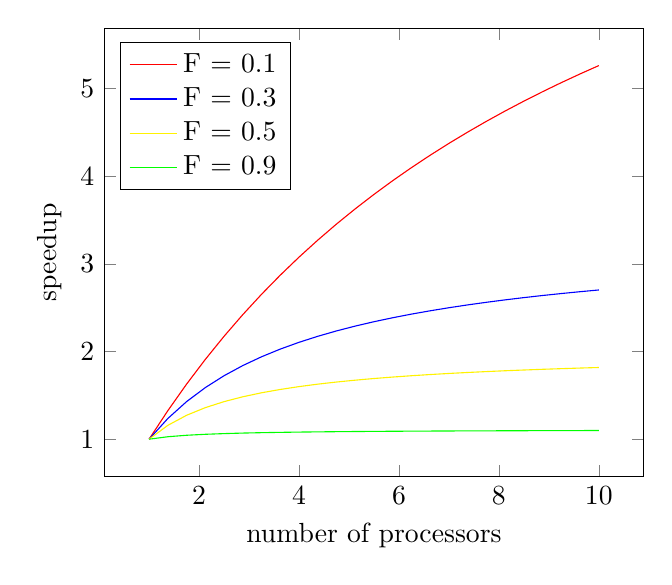
\begin{tikzpicture}
  \begin{axis}[
    xlabel = number of processors,
    ylabel =speedup,
    legend pos = north west,]
 \addplot[domain=1:10, color=red] {1/(0.1+(1-0.1)/x)}; 
 \addlegendentry{F = 0.1}
 \addplot[domain=1:10, color=blue] {1/(0.3+(1-0.3)/x)};
 \addlegendentry{F = 0.3}
 \addplot[domain=1:10, color=yellow] {1/(0.5+(1-0.5)/x)};
 \addlegendentry{F = 0.5}
 \addplot[domain=1:10, color=green] {1/(0.9+(1-0.9)/x)};
 \addlegendentry{F = 0.9}
 \end{axis}
\end{tikzpicture}
\label{fig:plot_cpu}

The graph shows how the performance gained by adding processors depends on the type of the computation. A computation that can not be parallelized much (high value of F) will have a low performance increase with more processors. 

\subsection{Balancing}

Let's consider a single CPU with multiple cores. To achieve the best possible performance the workload should be spread evenly between the cores, this means that there shouldn't be any core that does significantly less work than another. It is one of the job of the scheduler to keep the load of each core balanced. 

How is the load measured? The first option is to use the weights of the task. The load of a core is the sum of the weights of its tasks. But this doesn't work very well. Suppose that we have 4 tasks with the same priority, 2 are CPU intensive and 2 spend most of their time sleeping, and we want to balance the load between 2 processors. If we use only the weights of the tasks to balance, both the CPU intensive tasks could get assigned to one core, making it always busy, while the other core would be almost always idle as both of his tasks spend most of their time waiting.

The approach above doesn't take in consideration the nature of the tasks. An I/O bound task will spend a lot more time sleeping than a CPU intensive task. To effectively measure the load we need to keep track of the amount of time that a task spends sleeping. This wasn't necessary when we were considering a single processor. The load of a task is a combination of its weight and its average CPU utilization. And the load of the a core is the sum of the loads of its tasks. Since the CPU utilization of a task can vary, its load is constantly updated.

\subsubsection{Migrating tasks}
The scheduler periodically checks that the load of all the CPUs is balanced. In case it is not, the scheduler tries to migrate the tasks from one CPU to another in order to keep the balance. But the structure of the system plays an important role. The migration of a task could be expensive and, in some cases, it could be more efficient to not move the task.

In a simple multi-core CPU architecture there is one memory and the cost of accessing it is the same for all the cores. In this case the tasks can be migrated between cores without any constraints. But having a single memory is not efficient since two cores can not access the memory at the same time. 

Modern processors solve this problem by giving each core its own memory, but this creates a more complex structure. The cost of accessing the memory is no longer the same for all the cores, but depends on where the desired data is located. This means that migrating tasks between cores could lead to some overhead and sometimes it is more efficient to keep a task on the same core instead of moving it, even if the cores are not balanced. 

The same system could use a mix of the two structures. The cores could be divided in groups with their own memory. Accessing the memory of another group is more expensive. But inside a group all the cores can access the memory at same cost. Inside a group tasks can be migrated more frequently, while migration between groups should be less frequent. To efficiently use this structure the system gives the possibility of defining different migration policies.

\paragraph{Domains}
The structure of the system is described by two entities: scheduling domains and CPU groups. A scheduling domain is a set of CPUs, and a CPU group is a partition of the CPUs of a domain. A CPU inside a domain can not belong to two groups of the same domain and every CPU has to be part of a group. The scheduler does not balance the load between single CPUs, instead it tries to balance the loads among the CPU groups of a domain.

Let's take as example a system with 2 pairs of processors. A pair shares the same memory and its processors can exchange tasks without cost. On the other hand moving tasks between pairs is more expensive. This could represent a real scenario, where a pair represent as a single physical processor with inside two hyperthreaded CPUs.

Each pair is represented by a domain, which contains two CPU groups, one for each processor. The groups contains only one CPU in this case. Inside this domain balancing can happen very often since it can be done without additional cost. And the balancing is triggered by small differences in load between the groups of the domain.

To allow the tasks to be migrated from one domain to another, there is also an higher level domain that includes all the CPUs. It is partitioned in two two CPU groups, one for each pair. The two groups are kept balanced, but the scheduler does not try to balance the load inside a group. This domain tries to balance the load much less often and it is more tolerant to imbalances in the load.

There could also be other layers of domains. For example in a NUMA system there could be another domain representing a NUMA node, with a different migration policy.

Using this domain structure the scheduler can take in consideration the organization of the system when balancing the CPUs allowing for more efficient choices.